\chapter{Schwarzschild black hole}
\label{s:sch}
\index{Schwarzschild!black hole}

\minitoc

\section{Introduction}

After having discussed stationary black holes in Chap.~\ref{s:sta},
we examine here the simplest of them: the Schwarzschild black hole.
Let us recall the prime importance of the Schwarzschild black hole
in general relativity stems from the no-hair theorem (Sec.~\ref{s:sta:no-hair}),
which implies that any non-rotating black hole in an asymptotically flat
4-dimensional spacetime must a Schwarzschild black hole.

\section{The Schwarzschild-(anti-)de Sitter solution}

\subsection{Vacuum Einstein equation with a cosmological constant}

Let us search for a static and spherically symmetric solution of the
Einstein equation (\ref{e:bas:Einstein_eq}) in a vacuum
4-dimensional spacetime $(\M,\w{g})$ with some arbitrary cosmological constant
$\Lambda$. Setting $\w{T}=0$ in Eq.~(\ref{e:bas:Einstein_eq}) shows
that the equation to solve is
\be \label{e:sch:vac_Einstein_eq}
     \w{R} + \left(\Lambda - \frac{1}{2}\, R\right) \w{g} = 0 ,
\ee
$\w{R}$ being the Ricci tensor of $\w{g}$ and $R:=g^{\mu\nu} R_{\mu\nu}$ its
trace with respect to $\w{g}$, i.e. the so-called Ricci scalar
(cf. Sec.~\ref{s:bas:Ricci_tensor} in Appendix~\ref{s:bas}).
Let us first note that Eq.~(\ref{e:sch:vac_Einstein_eq}) implies a
constraint on the Ricci scalar. Indeed the trace of Eq.~(\ref{e:sch:vac_Einstein_eq})
with respect to $\w{g}$ is
\[
    R + \left(\Lambda - \frac{1}{2}\, R\right) \times 4 = 0 ,
\]
hence
\be \label{e:sch:R_4Lamb}
    \encadre{R = 4\Lambda} .
\ee
In particular the Ricci scalar is constant.
Inserting this value back into (\ref{e:sch:vac_Einstein_eq}), we get
\be \label{e:sch:vac_Einstein_eq_Lamb}
    \encadre{ \w{R} = \Lambda \, \w{g} } .
\ee
Since this equation yields (\ref{e:sch:R_4Lamb}) as well, we conclude
that it is equivalent to (\ref{e:sch:vac_Einstein_eq}).

\subsection{Static and spherically symmetric metric}

Let us assume that the spacetime $(\M,\w{g})$
is \defin{static}\index{static spacetime}, i.e. that it is
admits a Killing vector field $\w{\xi}$ that is timelike and
hypersurface-orthogonal (cf. Sec.~\ref{s:sta:staticity_thm}).
We may then foliate $\M$ by a 1-parameter family of hypersurfaces
$\left(\Sigma_t\right)_{t\in\R}$, such that $\w{\xi}$ is normal to
all $\Sigma_t$'s and $t$ is a parameter associated to $\w{\xi}$:
\be \label{e:sch:xi_t}
    \w{\xi}(t) = 1
\ee
or equivalently,
\[
    \langle \dd t , \w{\xi} \rangle = 1.
\]

In addition to be static, we assume that $(\M,\w{g})$ is \defin{spherically symmetric},
i.e. that it is invariant under the action of the rotation group $\mathrm{SO}(3)$,
whose orbits are spacelike 2-spheres (cf. Sec.~\ref{s:neh:symmetries}).
Let $\Sp$ be a generic orbit 2-sphere. The static Killing vector field $\w{\xi}$
must be orthogonal to $\Sp$, otherwise the orthogonal projection of $\w{\xi}$
onto $\Sp$ would define some privileged directions on $\Sp$, which is incompatible
with spherical symmetry. The orthogonality of $\w{\xi}$ and $\Sp$ implies
that $\Sp\subset\Sigma_t$. Let $(x^a)=(\th,\ph)$ be spherical coordinates on
$\Sp$. The metric $\w{q}$ induced by $\w{g}$ on $\Sp$ is given by
\be
    q_{ab}\, \D x^a\, \D x^b = r^2 \left( \D\th^2 + \sin^2\th\, \D\ph^2 \right) .
\ee
The coefficient $r^2$ in front of the standard spherical element must be
constant over $\Sp$, by virtue of spherical symmetry. The area of $\Sp$ is
then $A=4\pi r^2$. For this reason, $r$ is called the \defin{areal radius}\index{areal!radius}
of $\Sp$. Letting $\Sp$ vary, $r$ can be considered as a scalar field on
$\M$. If $\dd r \not = 0$, we may use it a coordinate. Since $\Sp\subset \Sigma_t$,
$(r,\th,\ph)$ is a coordinate system on each hypersurface $\Sigma_t$.
The set $(t,r,\th,\ph)$,
where $t$ is adapted to $\w{\xi}$ thanks to (\ref{e:sch:xi_t}) is then a
coordinate system and, by construction, the expression of the metric tensor
with respect to this system is
\be \label{e:sch:g_AB}
    g_{\mu\nu}\, \D x^\mu \, \D x^\nu = -A(r)\, \D t + B(r)\, \D r +
        r^2 \left( \D\th^2 + \sin^2\th\, \D\ph^2 \right) .
\ee
Note that in this coordinate system
\be
    \w{\xi} = \wpar_t
\ee
and that $g_{tt} = -A(r)$ and $g_{rr} = B(r)$ do not depend on $t$
as a result of the spacetime stationarity, while
$g_{tr} = g_{t\th} = g_{t\ph} = 0$ expresses the orthogonality of $\w{\xi}$
and $\Sigma_t$, i.e. the spacetime staticity.
The coordinates $(t,r,\th,\ph)$ are called \defin{areal coordinates}\index{areal!coordinates},
reflecting the fact that $r$ is the areal radius.

\subsection{Solving Einstein equation}

The Christoffel symbols of the metric (\ref{e:sch:g_AB}) with respect to the
areal coordinates are (cf. Sec.~\ref{s:sam:Kottler_solution} for the computation):
\be
\begin{array}{l}
\displaystyle  \Gamma^t_{\ \, tr} = \Gamma^t_{\ \, rt} = \frac{1}{2A}\derd{A}{r}\qquad
\Gamma^r_{\ \, tt} = \frac{1}{2B}\derd{A}{r} \qquad
\Gamma^r_{\ \, rr} = \frac{1}{2B}\derd{B}{r} \qquad
\Gamma^r_{\ \, \th\th} = -\frac{r}{B} \\[2ex]
\displaystyle  \Gamma^r_{\ \, \ph\ph} = -\frac{r\sin^2\th}{B} \qquad
\Gamma^\th_{\ \, r\th} = \Gamma^\th_{\ \, \th r} = \frac{1}{r} \qquad
\Gamma^\th_{\ \, \ph\ph} = -\sin\th\cos\th \\[2ex]
\displaystyle \Gamma^\ph_{\ \, r\ph} = \Gamma^\ph_{\ \, \ph r} = \frac{1}{r} \qquad
\Gamma^\ph_{\ \, \th\ph} = \Gamma^\ph_{\ \, \ph\th} = \frac{1}{\tan\th} ,
\end{array}
\ee
the Christoffel symbols not listed above being zero.

The $tt$ component of the Einstein equation (\ref{e:sch:vac_Einstein_eq})
leads to (cf. Sec.~\ref{s:sam:Kottler_solution} for the computation)
\be \label{e:sch:EE_tt}
        r \derd{B}{r} - B + (1 - \Lambda r^2) B^2 = 0 ,
\ee
while the $rr$ component leads to
\be \label{e:sch:EE_rr}
        r \derd{A}{r} + A - (1 - \Lambda r^2) AB = 0 .
\ee
Finally, the $\th\th$ and $\ph\ph$ components lead to the same equation:
\be
    2  \frac{\D^2 A}{\D r^2} + \frac{2}{r} \derd{A}{r}
        - \frac{1}{B} \left( \derd{A}{r} + \frac{2A}{r} \right) \derd{B}{r}
        - \frac{1}{A} \left( \derd{A}{r} \right) ^2
        + 4 \Lambda  A B  = 0 .
\ee
All the other components of the Einstein equation (\ref{e:sch:vac_Einstein_eq})
are identically zero.

Adding Eq.~(\ref{e:sch:EE_tt}) multiplied by $A$ to
Eq.~(\ref{e:sch:EE_rr}) multiplied by $B$ yields
\[
    B \derd{A}{r} + A \derd{B}{r} = \derd{}{r}(AB) = 0 .
\]
The solution of this equation is obviously $A(r)B(r) = C$, where $C$ is a constant.
Without any loss of generality, we may choose $C=1$. Indeed, substituting
$C/B(r)$ for $A(r)$ in Eq.~(\ref{e:sch:g_AB}) results in
\[
    g_{\mu\nu}\, \D x^\mu \, \D x^\nu = -\frac{C}{B(r)}\, \D t + B(r)\, \D r +
        r^2 \left( \D\th^2 + \sin^2\th\, \D\ph^2 \right) .
\]
Assuming $C>0$, the change of variable $t' = \sqrt{C} t$, which is equivalent
of changing the stationary Killing vector from $\w{\xi}$ to
$\w{\xi}'=  1/\sqrt{C}\, \w{\xi}$,
yields
\[
    g_{\mu\nu}\, \D x^\mu \, \D x^\nu = -\frac{1}{B(r)}\, \D t' + B(r)\, \D r +
        r^2 \left( \D\th^2 + \sin^2\th\, \D\ph^2 \right) ,
\]
which is exactly the solution corresponding to $C=1$. Hence from now on,
we set $C=1$, i.e.
\be
    B(r) = \frac{1}{A(r)} .
\ee
Substituting this expression in Eq.~(\ref{e:sch:EE_rr}) yields an ordinary
differential equation for $A(r)$:
\[
    r \derd{A}{r} + A - 1 + \Lambda r^2 = 0 ,
\]
the solution of which is
\be
    A(r) = 1 - \frac{2 m}{r} - \frac{\Lambda}{3} \,  r^2 ,
\ee
where $m$ is a constant.
The general static and spherically symmetric solution of the vacuum
Einstein equation (\ref{e:sch:vac_Einstein_eq}) is therefore
\be \label{e:sch:Kottler_metric}
    \encadre{
        g_{\mu\nu}\, \D x^\mu \, \D x^\nu =
            -\left( 1 - \frac{2 m}{r} - \frac{\Lambda}{3} \,  r^2\right)\, \D t
            + \left( 1 - \frac{2 m}{r} - \frac{\Lambda}{3} \,  r^2\right) ^{-1}\, \D r+
        r^2 \left( \D\th^2 + \sin^2\th\, \D\ph^2 \right) }.
\ee
It is called the \defin{Kottler metric}\index{Kottler metric}. The particular case $\Lambda=0$
is called the \defin{Schwarzschild metric}\index{Schwarzschild!metric}. If $\Lambda>0$,
(\ref{e:sch:Kottler_metric}) is called the
\defin{Schwarzschild-de Sitter metric}\index{Schwarzschild!de Sitter metric},
often abridged as \defin{Schwarzschild-dS metric}, while if $\Lambda<0$, it
is called the \defin{Schwarzschild-anti-de Sitter metric}\index{Schwarzschild!anti-de Sitter metric},
often abridged as \defin{Schwarzschild-AdS metric}\index{Schwarzschild!AdS metric}.

In the rest of this chapter, we will focuss on the Schwarzschild metric,
i.e. the version $\Lambda=0$ of Eq.~(\ref{e:sch:Kottler_metric}):
\be \label{e:sch:Schwarz_metric_SD}
    \encadre{
        g_{\mu\nu}\, \D x^\mu \, \D x^\nu =
            -\left( 1 - \frac{2 m}{r} \right)\, \D t
            + \left( 1 - \frac{2 m}{r} \right) ^{-1}\, \D r +
        r^2 \left( \D\th^2 + \sin^2\th\, \D\ph^2 \right) }.
\ee
The coordinates $(t,r,\th,\ph)$ are then called
\defin{Schwarzschild-Droste coordinates}\index{Schwarzschild-Droste coordinates}\footnote{In the literature they are commonly referred to as simply
\defin{Schwarzschild coordinates}\index{Schwarzschild!coordinates}.}.

\begin{hist}
The Schwarzschild metric (\ref{e:sch:Schwarz_metric_SD}) is actually
the first non-trivial (i.e. different from Minkowski metric) solution
of Einstein equation ever found. It has been obtained by the
astrophysicist Karl Schwarzchild in the end of 1915 \cite{Schwa1916}, only a few weeks
after the publication of the articles funding general relativity by
Albert Einstein. It is also quite remarkable that
Schwarzschild found the solution while serving in the German army at the Russian
front. Unfortunately, he died from a rare skin disease a few month later.
The way Schwarzschild proceeded was quite different from that exposed above:
instead of the coordinates $(t,r,\th,\ph)$
named today after him, he used the coordinates
$(t,x^1,x^2,\ph)$ where $x^1 = r_*^3/3$, with $r_*^3 = r^3-8m^3$, and
$x^2 = -\cos\th$. Such a choice was made to enforce $\det\w{g} = -1$, a condition
prescribed by Einstein in an early version of general relativity, which had been presented on
18 November 2015 and on which Schwarzschild was working on. Only in the final version, published on
25 November 2015, did Einstein relax the condition $\det\w{g} = -1$, allowing for full
covariance. Schwarzschild however
exhibited the line element (\ref{e:sch:Schwarz_metric_SD}), via what he
called the ``auxiliary quantity'' $r = (r_*^3 + 8m^3)^{1/3}$.
For him, the ``center'',  namely the location of the ``point mass'' generating the field,
was at $r_* = 0$, i.e. at $r=2m$.
Independently of Schwarzschild, Johannes Droste, then PhD student of
Hendrik Lorentz,
arrives at the solution (\ref{e:sch:Schwarz_metric_SD}) in May 1916 \cite{Drost1917}.
Contrary to Schwarzschild, Droste performed the computation with
a spherical coordinate system, $(t,\bar r, \th,\ph)$, yet distinct from
the standard ``Schwarzschild-Droste'' coordinates $(t,r,\th,\ph)$ by the fact that the radial
coordinate $\bar r$ was not chosen to be the areal radius, but instead a
coodinate for which $g_{\bar r\bar r} = 1$. At the end, by a change of
variable, Droste exhibited the solution (\ref{e:sch:Schwarz_metric_SD}).
The generalization to a non-vanishing cosmological constant, i.e.
Eq.~(\ref{e:sch:Kottler_metric}) has been obtained by
Friedrich Kottler in 1918 \cite{Kottl1918} and, independently, by
Hermann Weyl in 1919 \cite{Weyl1919}. We refer to the article by Eisenstaedt
\cite{Eisen82} for a detailed account of the early history of the
Schwarzschild solution.
\end{hist}

%%%%%%%%%%%%%%%%%%%%%%%%%%%%%%%%%%%%%%%%%%%%%%%%%%%%%%%%%%%%%%%%%%%%%%%%%%%%%%%

\section{The Schwarzschild-Droste spacetime}

\subsection{The Schwarzschild-Droste manifold}

We immediately notice on (\ref{e:sch:Schwarz_metric_SD}) that the metric
components are singular at $r=0$ and $r=2m$. Accordingly, the Schwarzschild-Droste coordinates $(t,r,\th,\ph)$ cover the following manifold, made of two connected components:
\begin{subequations}
\begin{align}
    \M_{\rm SB} & :=  \M_{\rm I} \cup \M_{\rm II} , \\
    \M_{\rm I} & :=  \R\times(2m,+\infty)\times\SS^2 ,\\
    \M_{\rm II} & :=  \R\times(0,2m)\times\SS^2 ,
\end{align}
\end{subequations}
with the coordinate $t$ spanning $\R$, the coordinate $r$ spanning $(2m,+\infty)$
on $M_{\rm I}$ and $(0,2m)$ on $M_{\rm II}$, and the coordinates $(\th,\ph)$
constituting the standard spherical chart of $\SS^2$.


\subsection{Basic properties}



%%%%%%%%%%%%%%%%%%%%%%%%%%%%%%%%%%%%%%%%%%%%%%%%%%%%%%%%%%%%%%%%%%%%%%%%%%%%%%%

\section{Radial null geodesics}

\subsection{Determination of the radial null geodesics}

Let us search for null geodesics of the Schwarzschild metric
(\ref{e:sch:Schwarz_metric_SD}) that are radial, i.e. along which
$\th=\mathrm{const}$ and $\ph=\mathrm{const}$. They are found by
setting  $\D\th=0$ and $\D\ph=0$
in (\ref{e:sch:Schwarz_metric_SD})
and searching for $\D s^2 = g_{\mu\nu}\, \D x^\mu \, \D x^\nu = 0$:
\[
    \D s^2 = 0 \iff \D t^2 = \frac{\D r^2}{\left( 1 - \frac{2m}{r} \right) ^2} .
\]
Hence the radial null geodesics are governed by
\be
    \D t = \pm \frac{\D r}{ 1 - \frac{2m}{r} } .
\ee
This equation is easily integrated, yielding
\be
    t = \pm r \pm 2 m \ln \left| \frac{r}{2m} - 1 \right| + \mathrm{const} .
\ee
We have thus two families of radial null geodesics, one for each choice
of sign in the $\pm$:

\begin{figure}
\centerline{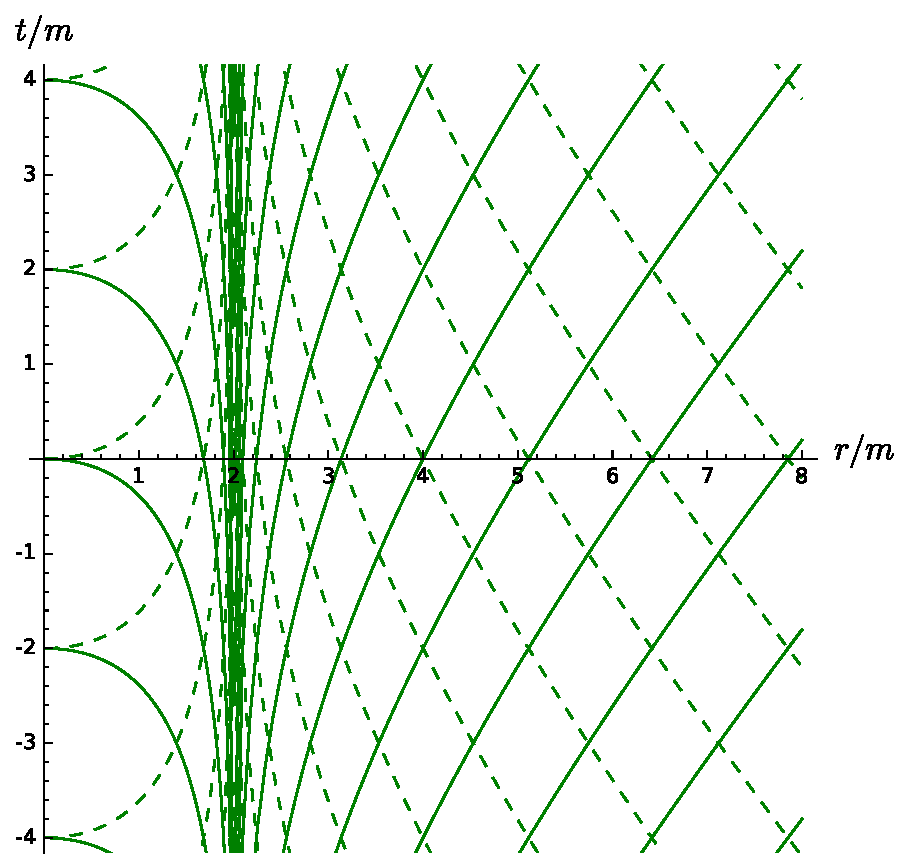
\includegraphics[width=0.6\textwidth]{sch_rad_null_geod.pdf}}
\caption[]{\label{f:sch:rad_null_geod} \footnotesize
Radial null geodesics of Schwarzschild spacetime, plotted in terms
of Schwarzschild-Droste coordinates $(t,r)$: the solid (resp. dashed) lines
correspond to outgoing (resp. ingoing) geodesics, as given by Eq.~(\ref{e:sch:outgoing_null_geod})
(resp. Eq.~(\ref{e:sch:ingoing_null_geod}). The interiors of some future light
cones are drawn in yellow.}
\end{figure}

\begin{itemize}
\item the \defin{outgoing radial null geodesics}\index{outgoing!null geodesic}, whose
equation is
\be \label{e:sch:outgoing_null_geod}
    t = r + 2 m \ln \left| \frac{r}{2m} - 1 \right| + u ,
\ee
where $u$ is a constant;
\item  the \defin{ingoing radial null geodesics}\index{ingoing!null geodesic}, whose
equation is
\be \label{e:sch:ingoing_null_geod}
    t = - r - 2 m \ln \left| \frac{r}{2m} - 1 \right| + v ,
\ee
where $v$ is a constant.
\end{itemize}
These two families are depicted in Fig.~\ref{f:sch:rad_null_geod}.
The singularity of Schwarzschild-Droste coordinates at $r=2m$
is clearly apparent on this figure.

\begin{remark}
Despite their name, gedeosics of the outgoing family are actually
\emph{ingoing} in the region $r<2m$, in the sense that
$r$ is decreasing along them when moving towards the future. Indeed,
for $r<2m$, $r$ is the timelike coordinate of the system $(t,r,\th,\ph)$,
with $-\wpar_r$ oriented towards the future (cf. the ``tilted'' light cone
in Fig.~\ref{f:sch:rad_null_geod}).
\end{remark}

%%%%%%%%%%%%%%%%%%%%%%%%%%%%%%%%%%%%%%%%%%%%%%%%%%%%%%%%%%%%%%%%%%%%%%%%%%%%%%%

\section{Maximal extension}

\begin{figure}
\centerline{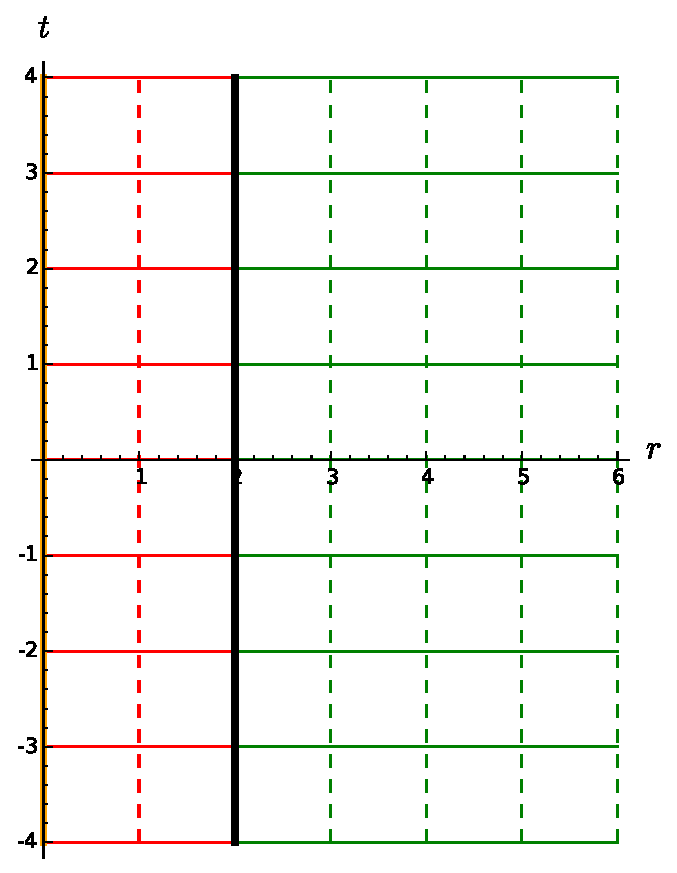
\includegraphics[height=0.37\textheight]{sch_coord_schwarz.pdf}\qquad
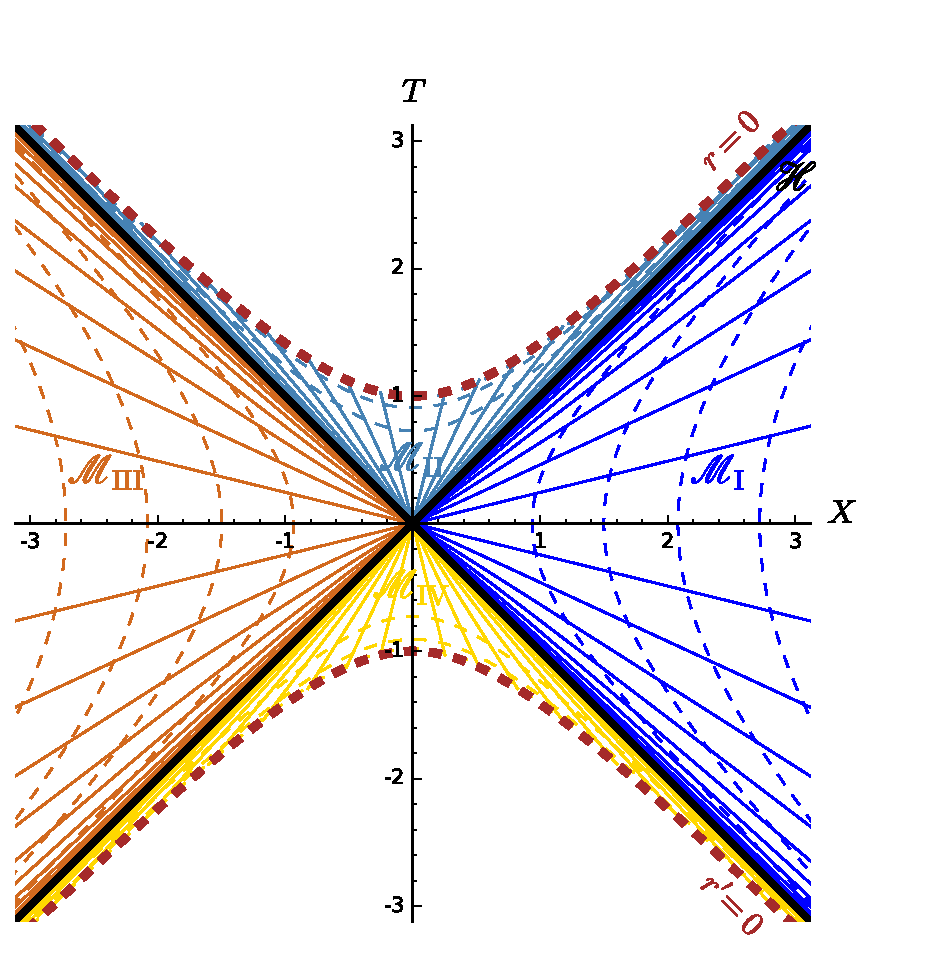
\includegraphics[height=0.37\textheight]{sch_kruskal_diag.pdf}}
\caption[]{\label{f:sch:kruskal_diag} \footnotesize
Schwarzschild spacetime depicted in Schwarzschild-Droste coordinates $(t,r)$
(left) and in Kruskal-Szekeres coordinates $(T,X)$ (right). In both figures,
green (resp. red) solid curves denote the hypersurfaces $t=\mathrm{const}$
in Region~I (resp. II), while green (resp. red) dashed curves
denote the hypersurfaces $r=\mathrm{const}$ in Region~I (resp. II).
The future and past event horizons are marked by thick black lines, while the
singularity at $r=0$ is depicted in orange. Regions III and IV are depicted
in grey and pink respectively. Note that the left figure covers only Regions I and II.}
\end{figure}

\begin{figure}
\centerline{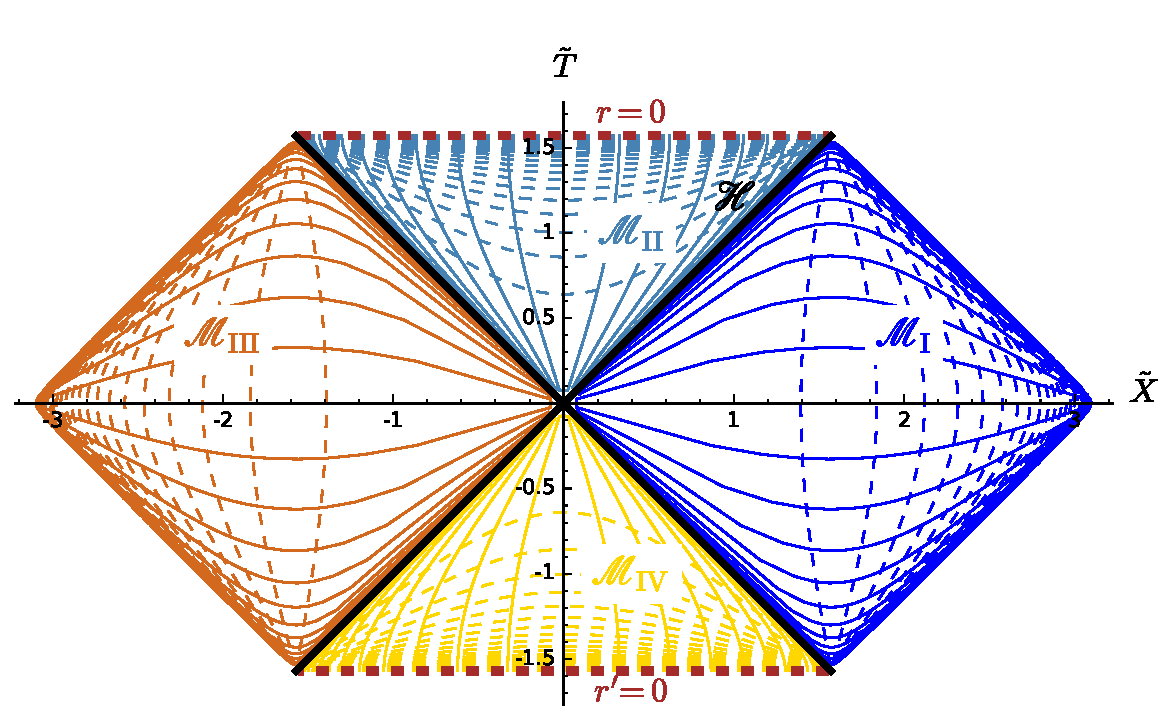
\includegraphics[width=0.9\textwidth]{sch_carter-penrose.pdf}}
\caption[]{\label{f:sch:sch_carter-penrose} \footnotesize
Schwarzschild spacetime depicted in Carter-Penrose coordinates $(\tilde{T},\tilde{X})$; the color code
is the same as in Fig.~\ref{f:sch:kruskal_diag}.
As Fig.~\ref{f:sch:kruskal_diag}, this figure has been produced with
SageManifolds (cf. Appendix~\ref{s:sam}).}
\end{figure}

